% Options for packages loaded elsewhere
\PassOptionsToPackage{unicode}{hyperref}
\PassOptionsToPackage{hyphens}{url}
\PassOptionsToPackage{dvipsnames,svgnames,x11names}{xcolor}
%
\documentclass[
  letterpaper,
  DIV=11,
  numbers=noendperiod]{scrartcl}

\usepackage{amsmath,amssymb}
\usepackage{lmodern}
\usepackage{iftex}
\ifPDFTeX
  \usepackage[T1]{fontenc}
  \usepackage[utf8]{inputenc}
  \usepackage{textcomp} % provide euro and other symbols
\else % if luatex or xetex
  \usepackage{unicode-math}
  \defaultfontfeatures{Scale=MatchLowercase}
  \defaultfontfeatures[\rmfamily]{Ligatures=TeX,Scale=1}
\fi
% Use upquote if available, for straight quotes in verbatim environments
\IfFileExists{upquote.sty}{\usepackage{upquote}}{}
\IfFileExists{microtype.sty}{% use microtype if available
  \usepackage[]{microtype}
  \UseMicrotypeSet[protrusion]{basicmath} % disable protrusion for tt fonts
}{}
\makeatletter
\@ifundefined{KOMAClassName}{% if non-KOMA class
  \IfFileExists{parskip.sty}{%
    \usepackage{parskip}
  }{% else
    \setlength{\parindent}{0pt}
    \setlength{\parskip}{6pt plus 2pt minus 1pt}}
}{% if KOMA class
  \KOMAoptions{parskip=half}}
\makeatother
\usepackage{xcolor}
\setlength{\emergencystretch}{3em} % prevent overfull lines
\setcounter{secnumdepth}{-\maxdimen} % remove section numbering
% Make \paragraph and \subparagraph free-standing
\ifx\paragraph\undefined\else
  \let\oldparagraph\paragraph
  \renewcommand{\paragraph}[1]{\oldparagraph{#1}\mbox{}}
\fi
\ifx\subparagraph\undefined\else
  \let\oldsubparagraph\subparagraph
  \renewcommand{\subparagraph}[1]{\oldsubparagraph{#1}\mbox{}}
\fi

\usepackage{color}
\usepackage{fancyvrb}
\newcommand{\VerbBar}{|}
\newcommand{\VERB}{\Verb[commandchars=\\\{\}]}
\DefineVerbatimEnvironment{Highlighting}{Verbatim}{commandchars=\\\{\}}
% Add ',fontsize=\small' for more characters per line
\usepackage{framed}
\definecolor{shadecolor}{RGB}{241,243,245}
\newenvironment{Shaded}{\begin{snugshade}}{\end{snugshade}}
\newcommand{\AlertTok}[1]{\textcolor[rgb]{0.68,0.00,0.00}{#1}}
\newcommand{\AnnotationTok}[1]{\textcolor[rgb]{0.37,0.37,0.37}{#1}}
\newcommand{\AttributeTok}[1]{\textcolor[rgb]{0.40,0.45,0.13}{#1}}
\newcommand{\BaseNTok}[1]{\textcolor[rgb]{0.68,0.00,0.00}{#1}}
\newcommand{\BuiltInTok}[1]{\textcolor[rgb]{0.00,0.23,0.31}{#1}}
\newcommand{\CharTok}[1]{\textcolor[rgb]{0.13,0.47,0.30}{#1}}
\newcommand{\CommentTok}[1]{\textcolor[rgb]{0.37,0.37,0.37}{#1}}
\newcommand{\CommentVarTok}[1]{\textcolor[rgb]{0.37,0.37,0.37}{\textit{#1}}}
\newcommand{\ConstantTok}[1]{\textcolor[rgb]{0.56,0.35,0.01}{#1}}
\newcommand{\ControlFlowTok}[1]{\textcolor[rgb]{0.00,0.23,0.31}{#1}}
\newcommand{\DataTypeTok}[1]{\textcolor[rgb]{0.68,0.00,0.00}{#1}}
\newcommand{\DecValTok}[1]{\textcolor[rgb]{0.68,0.00,0.00}{#1}}
\newcommand{\DocumentationTok}[1]{\textcolor[rgb]{0.37,0.37,0.37}{\textit{#1}}}
\newcommand{\ErrorTok}[1]{\textcolor[rgb]{0.68,0.00,0.00}{#1}}
\newcommand{\ExtensionTok}[1]{\textcolor[rgb]{0.00,0.23,0.31}{#1}}
\newcommand{\FloatTok}[1]{\textcolor[rgb]{0.68,0.00,0.00}{#1}}
\newcommand{\FunctionTok}[1]{\textcolor[rgb]{0.28,0.35,0.67}{#1}}
\newcommand{\ImportTok}[1]{\textcolor[rgb]{0.00,0.46,0.62}{#1}}
\newcommand{\InformationTok}[1]{\textcolor[rgb]{0.37,0.37,0.37}{#1}}
\newcommand{\KeywordTok}[1]{\textcolor[rgb]{0.00,0.23,0.31}{#1}}
\newcommand{\NormalTok}[1]{\textcolor[rgb]{0.00,0.23,0.31}{#1}}
\newcommand{\OperatorTok}[1]{\textcolor[rgb]{0.37,0.37,0.37}{#1}}
\newcommand{\OtherTok}[1]{\textcolor[rgb]{0.00,0.23,0.31}{#1}}
\newcommand{\PreprocessorTok}[1]{\textcolor[rgb]{0.68,0.00,0.00}{#1}}
\newcommand{\RegionMarkerTok}[1]{\textcolor[rgb]{0.00,0.23,0.31}{#1}}
\newcommand{\SpecialCharTok}[1]{\textcolor[rgb]{0.37,0.37,0.37}{#1}}
\newcommand{\SpecialStringTok}[1]{\textcolor[rgb]{0.13,0.47,0.30}{#1}}
\newcommand{\StringTok}[1]{\textcolor[rgb]{0.13,0.47,0.30}{#1}}
\newcommand{\VariableTok}[1]{\textcolor[rgb]{0.07,0.07,0.07}{#1}}
\newcommand{\VerbatimStringTok}[1]{\textcolor[rgb]{0.13,0.47,0.30}{#1}}
\newcommand{\WarningTok}[1]{\textcolor[rgb]{0.37,0.37,0.37}{\textit{#1}}}

\providecommand{\tightlist}{%
  \setlength{\itemsep}{0pt}\setlength{\parskip}{0pt}}\usepackage{longtable,booktabs,array}
\usepackage{calc} % for calculating minipage widths
% Correct order of tables after \paragraph or \subparagraph
\usepackage{etoolbox}
\makeatletter
\patchcmd\longtable{\par}{\if@noskipsec\mbox{}\fi\par}{}{}
\makeatother
% Allow footnotes in longtable head/foot
\IfFileExists{footnotehyper.sty}{\usepackage{footnotehyper}}{\usepackage{footnote}}
\makesavenoteenv{longtable}
\usepackage{graphicx}
\makeatletter
\def\maxwidth{\ifdim\Gin@nat@width>\linewidth\linewidth\else\Gin@nat@width\fi}
\def\maxheight{\ifdim\Gin@nat@height>\textheight\textheight\else\Gin@nat@height\fi}
\makeatother
% Scale images if necessary, so that they will not overflow the page
% margins by default, and it is still possible to overwrite the defaults
% using explicit options in \includegraphics[width, height, ...]{}
\setkeys{Gin}{width=\maxwidth,height=\maxheight,keepaspectratio}
% Set default figure placement to htbp
\makeatletter
\def\fps@figure{htbp}
\makeatother

\KOMAoption{captions}{tableheading}
\makeatletter
\@ifpackageloaded{tcolorbox}{}{\usepackage[many]{tcolorbox}}
\@ifpackageloaded{fontawesome5}{}{\usepackage{fontawesome5}}
\definecolor{quarto-callout-color}{HTML}{909090}
\definecolor{quarto-callout-note-color}{HTML}{0758E5}
\definecolor{quarto-callout-important-color}{HTML}{CC1914}
\definecolor{quarto-callout-warning-color}{HTML}{EB9113}
\definecolor{quarto-callout-tip-color}{HTML}{00A047}
\definecolor{quarto-callout-caution-color}{HTML}{FC5300}
\definecolor{quarto-callout-color-frame}{HTML}{acacac}
\definecolor{quarto-callout-note-color-frame}{HTML}{4582ec}
\definecolor{quarto-callout-important-color-frame}{HTML}{d9534f}
\definecolor{quarto-callout-warning-color-frame}{HTML}{f0ad4e}
\definecolor{quarto-callout-tip-color-frame}{HTML}{02b875}
\definecolor{quarto-callout-caution-color-frame}{HTML}{fd7e14}
\makeatother
\makeatletter
\makeatother
\makeatletter
\makeatother
\makeatletter
\@ifpackageloaded{caption}{}{\usepackage{caption}}
\AtBeginDocument{%
\ifdefined\contentsname
  \renewcommand*\contentsname{Table of contents}
\else
  \newcommand\contentsname{Table of contents}
\fi
\ifdefined\listfigurename
  \renewcommand*\listfigurename{List of Figures}
\else
  \newcommand\listfigurename{List of Figures}
\fi
\ifdefined\listtablename
  \renewcommand*\listtablename{List of Tables}
\else
  \newcommand\listtablename{List of Tables}
\fi
\ifdefined\figurename
  \renewcommand*\figurename{Figure}
\else
  \newcommand\figurename{Figure}
\fi
\ifdefined\tablename
  \renewcommand*\tablename{Table}
\else
  \newcommand\tablename{Table}
\fi
}
\@ifpackageloaded{float}{}{\usepackage{float}}
\floatstyle{ruled}
\@ifundefined{c@chapter}{\newfloat{codelisting}{h}{lop}}{\newfloat{codelisting}{h}{lop}[chapter]}
\floatname{codelisting}{Listing}
\newcommand*\listoflistings{\listof{codelisting}{List of Listings}}
\makeatother
\makeatletter
\@ifpackageloaded{caption}{}{\usepackage{caption}}
\@ifpackageloaded{subcaption}{}{\usepackage{subcaption}}
\makeatother
\makeatletter
\@ifpackageloaded{tcolorbox}{}{\usepackage[many]{tcolorbox}}
\makeatother
\makeatletter
\@ifundefined{shadecolor}{\definecolor{shadecolor}{rgb}{.97, .97, .97}}
\makeatother
\makeatletter
\makeatother
\ifLuaTeX
  \usepackage{selnolig}  % disable illegal ligatures
\fi
\IfFileExists{bookmark.sty}{\usepackage{bookmark}}{\usepackage{hyperref}}
\IfFileExists{xurl.sty}{\usepackage{xurl}}{} % add URL line breaks if available
\urlstyle{same} % disable monospaced font for URLs
\hypersetup{
  colorlinks=true,
  linkcolor={blue},
  filecolor={Maroon},
  citecolor={Blue},
  urlcolor={Blue},
  pdfcreator={LaTeX via pandoc}}

\author{}
\date{}

\begin{document}
\ifdefined\Shaded\renewenvironment{Shaded}{\begin{tcolorbox}[interior hidden, borderline west={3pt}{0pt}{shadecolor}, enhanced, breakable, frame hidden, boxrule=0pt, sharp corners]}{\end{tcolorbox}}\fi

\hypertarget{grunnleggende}{%
\section{Det grunnleggende}\label{grunnleggende}}

Vi starter gradvis på bunnen og arbeider oss kjapt opp til den avanserte
arbeidsflyten vi er vant med. Det vil si at vi starter med enkle lister
og datasett. Så forlater vi dette og jobber kun med datasett.

\begin{Shaded}
\begin{Highlighting}[]
\CommentTok{\# Laster inn tidyverse, som vi alltid bruker}
\FunctionTok{library}\NormalTok{(tidyverse)}
\end{Highlighting}
\end{Shaded}

\begin{verbatim}
-- Attaching packages --------------------------------------- tidyverse 1.3.2 --
v ggplot2 3.3.6      v purrr   0.3.5 
v tibble  3.1.8      v dplyr   1.0.10
v tidyr   1.2.1      v stringr 1.4.1 
v readr   2.1.3      v forcats 0.5.2 
-- Conflicts ------------------------------------------ tidyverse_conflicts() --
x dplyr::filter() masks stats::filter()
x dplyr::lag()    masks stats::lag()
\end{verbatim}

\hypertarget{sec-rstudio}{%
\subsection{Rstudio}\label{sec-rstudio}}

Men først av alt bør vi ta en titt på Rstudio. Dette er som nevnt det
grafiske brukergrensesnittet som vi arbeider i når vi jobber med R. Et
typisk Rstudio-vindu kan se slik ut:

\begin{figure}

{\centering 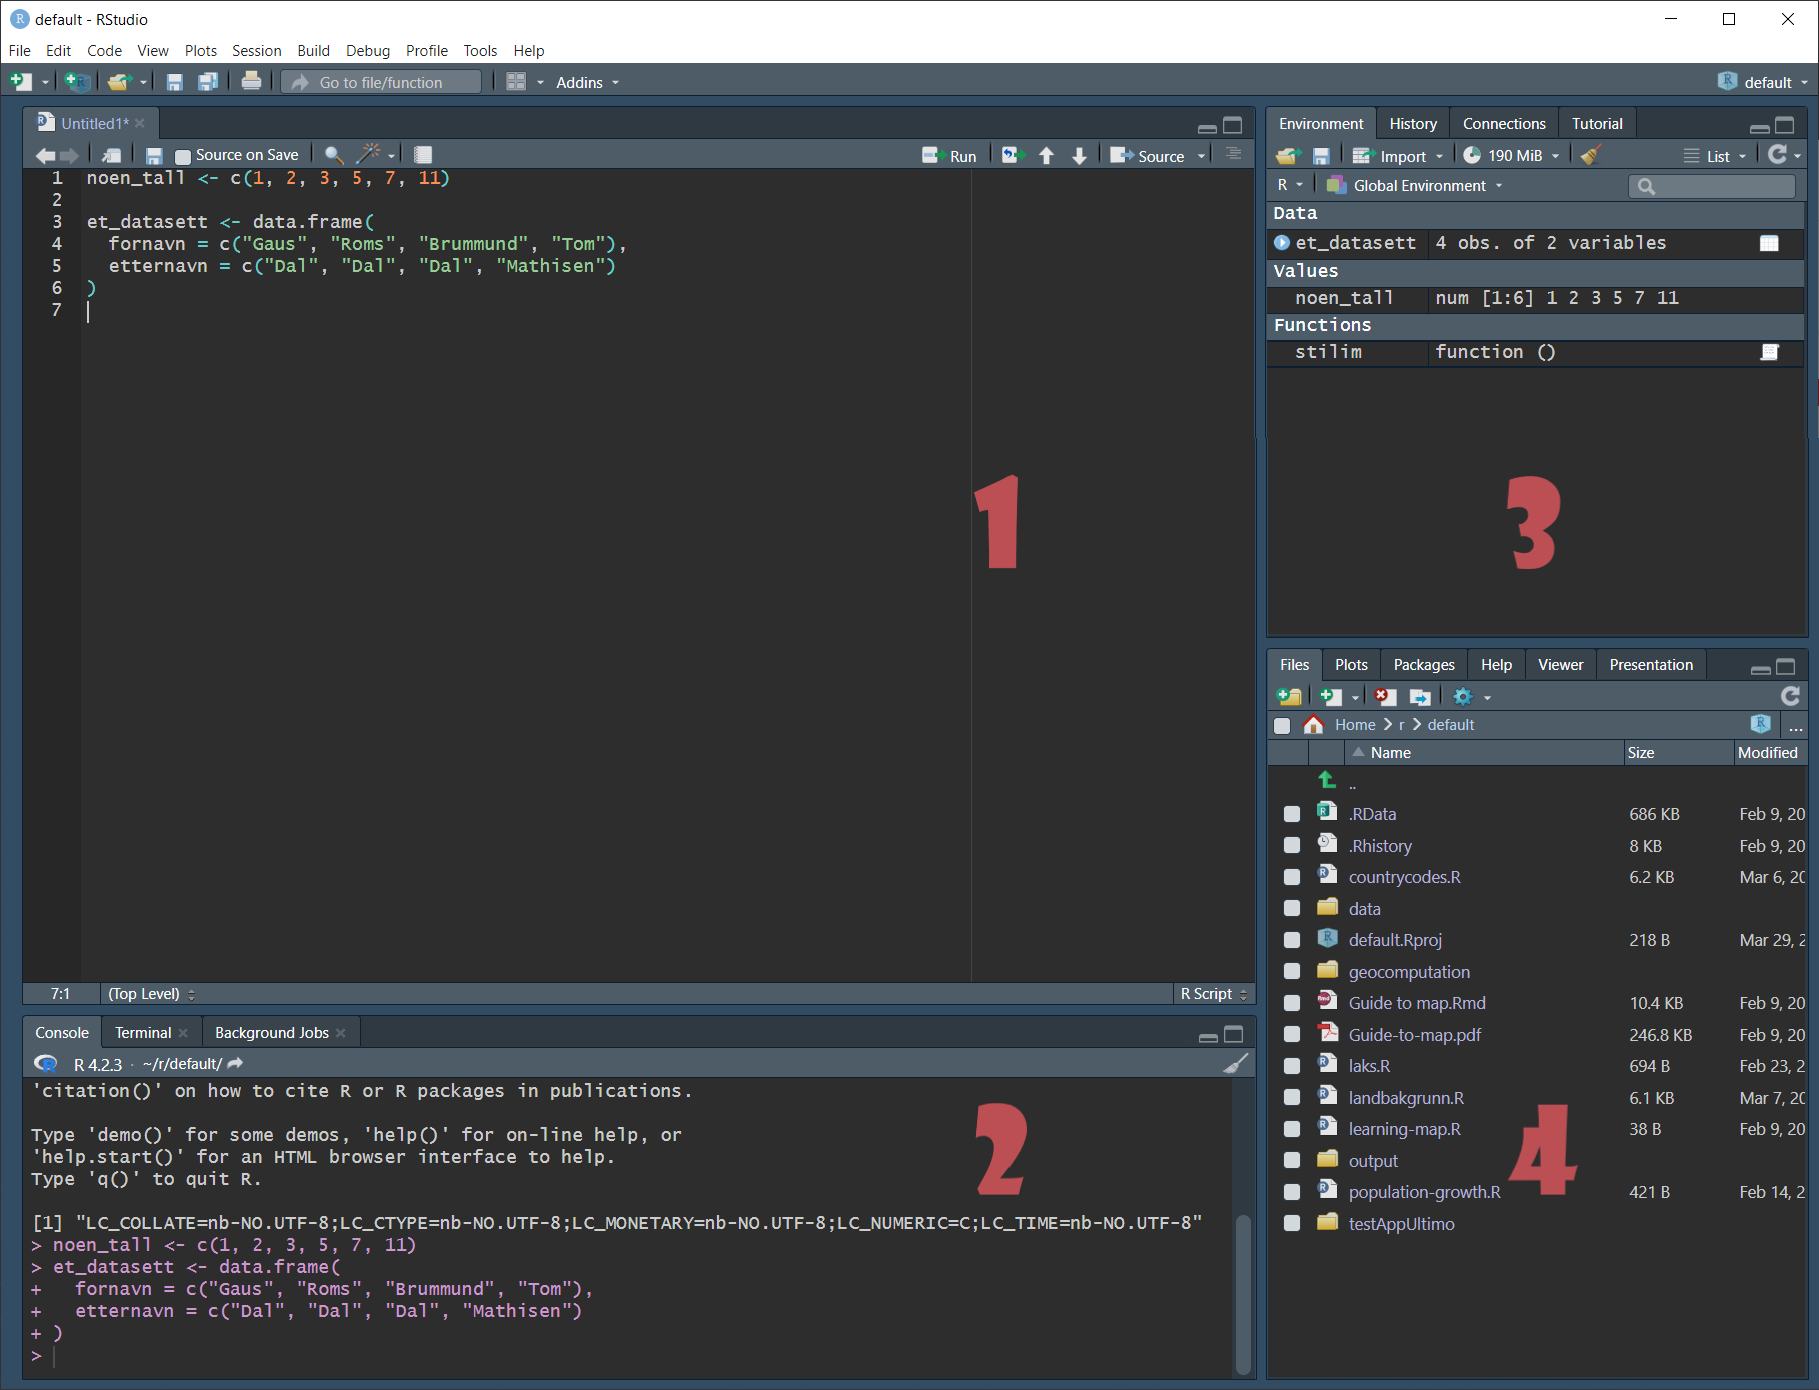
\includegraphics{img/rstudio_annotated.PNG}

}

\caption{Rstudio in action, med tema \emph{Tomorrow Night 80s}}

\end{figure}

Hvis du har kjedeligere farger er det nok fordi du ikke har oppdaga de
flotte temaene som du kan velge mellom i Rstudio. Kikk på
\emph{Tools/Global options/Appearance} og endre \emph{Editor theme} til
noe som faller deg i smak. Min favoritt for tida er \emph{Tomorrow Night
80s}. Grensesnittet består av fire ruter (\emph{panes}), som hver kan ha
flere faner (\emph{tabs}).

Når du først er i innstillinger: Skru av \emph{Restore .RData into
workspace on startup} og velg \emph{never} på \emph{Save workspace to
.RData on exit}. Dette er innstillinger som gjør det litt raskere for
deg å komme inn i et prosjekt, men som vil gi deg en falsk trygghet, og
som inviterer til noen av de feilene om jeg omtaler i
\textbf{?@sec-feil}. Derfor skrur vi dem av.\footnote{Hvorfor skrur vi
  av dette? Innstillinga er på \emph{by default} og vil lagre alt som
  ligger i miljøet ditt mellom hver gang du jobber i Rstudio, sjøl om du
  lukker programmet og skrur av maskina. Dette gjør det som nevnt
  lettere å starte opp igjen. Samtidig fører det til at miljøet ditt
  blir overfylt av gamle objekter og pakker du har lasta inn. Du kommer
  til å på et tidspunkt få en feil fordi du har lasta inn en gammel
  pakke du hadde glemt, eller fordi det ligger et objekt i miljøet du
  hadde glemt av. Det er god hygiene å restarte sesjonen ofte (flere
  ganger i løpet av et prosjekt), og denne innstillinga er med på å
  hindre deg i å gjøre det.}

\begin{figure}

{\centering 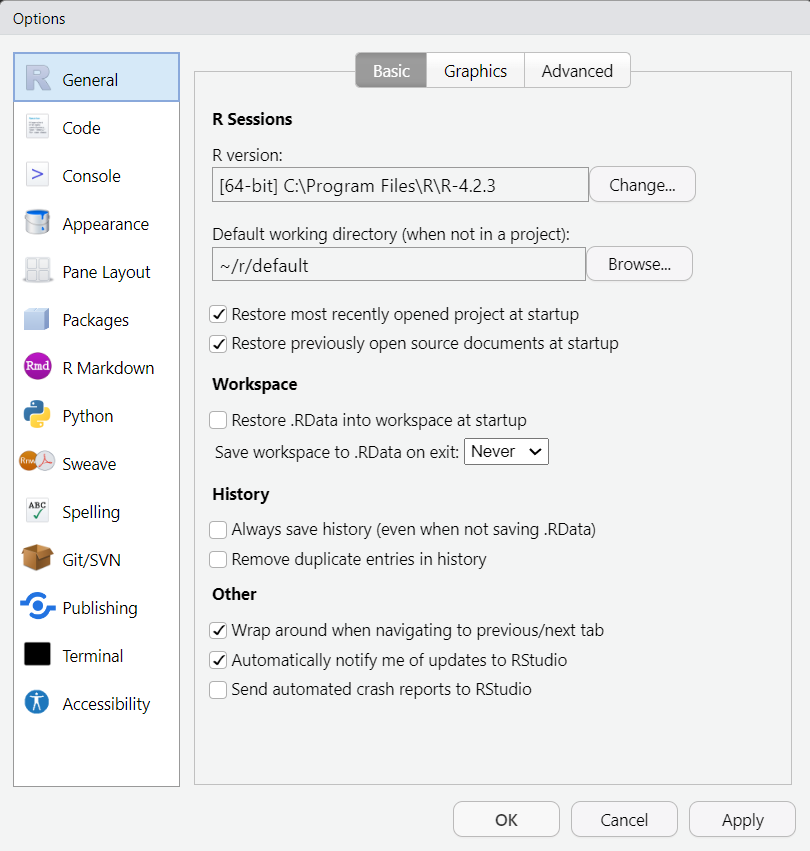
\includegraphics[width=0.5\textwidth,height=\textheight]{img/settings.png}

}

\caption{Slik skal det se ut}

\end{figure}

\hypertarget{rute-1-kilde-source}{%
\subsubsection{\texorpdfstring{Rute 1: Kilde
(\emph{source})}{Rute 1: Kilde (source)}}\label{rute-1-kilde-source}}

I denne ruta havner alle skriptene våre. Vi skriver alle kommandoene
våre i skript som vi deretter kjører. Dette er likt hvordan
syntaks/skript kan brukes i Stata og SPSS. Disse skripta blir en
oppskrift for oss seinere som forteller oss hva som blei gjort. Du kan
kjøre ei og ei linje ved å trykke \texttt{ctrl\ +\ enter}\footnote{For
  macOS-brukere: erstatt \texttt{ctrl} med \texttt{cmd} i disse
  snarveiene.}, eller du kan markere det du vil kjøre og trykke det
samme. Du kan kjøre hele skriptet ved å trykke
\texttt{ctrl\ +\ alt\ +\ enter}. Skript lar deg enkelt dele arbeidet
ditt med andre. Du bør være flink på å \emph{dokumentere} det du gjør
ved å bruke kommentarer. Dette er linjer som starter med \texttt{\#}.
Disse linjene vil ignoreres av R når du kjører skriptet.

Du kan se at jeg har skrevet noe kode i skriptet mitt. Jeg lager en
vektor som heter \emph{noen\_tall} og et datasett som heter
\emph{et\_datasett}.

\hypertarget{rute-2-konsollen-console}{%
\subsubsection{\texorpdfstring{Rute 2: Konsollen
(\emph{console})}{Rute 2: Konsollen (console)}}\label{rute-2-konsollen-console}}

Man kan også skrive kommandoer rett til konsollen. Da blir de kjørt med
en gang man trykker \texttt{enter}. De kodene du skriver til konsollen
vil ikke bli lagra noe sted, så hvis du jobber mye her vil du ikke
dokumentere arbeidet ditt. Så ikke gjør det til en vane å bruke
konsollen mye. Den er nyttig hvis du veit at du ikke trenger å ta vare
på akkurat det du gjør nå. F.eks. hvis du skal regne ut noe fort, eller
printe et objekt for å inspisere det.

Når du kjører skript vil koden skrives ut til konsollen. Du kan se at
jeg har kjørt kodene i skriptet fordi de er blitt skrevet til konsollen.

\hypertarget{rute-3-miljuxf8et-environment-med-mer}{%
\subsubsection{\texorpdfstring{Rute 3: Miljøet (\emph{environment}) med
mer}{Rute 3: Miljøet (environment) med mer}}\label{rute-3-miljuxf8et-environment-med-mer}}

De to siste rutene kan inneholde diverse faner, avhengig av hva du
krysser av for i \emph{Pane layout} i \emph{global options}. Vanligvis
viser det oss miljøet vårt. Her finner du en oversikt over alle
objektene du har laga hittil i \textbf{sesjonen} (\emph{session}) din.
En sesjon starter når du starter R (som starter når du starter Rstudio).
Den varer til du skrur av R eller restarter den manuelt. Du restarter
den manuelt ved å gå til \emph{Session/Restart R} eller trykke
\texttt{ctrl\ +\ shift\ +\ F10}.

Du kan se at det ligger en vektor, et datasett og en funksjon
(\emph{stilim()}) i mijøet mitt. De to første er det jeg lagde i
skriptet. Da koden blei kjørt lagde de to \textbf{objekter} (et datasett
og en vektor), og alle objekter legges i miljøet. Funksjonen ligger der
fordi den er definert i min \emph{.Rprofile}. Dette går jeg ikke inn på
her, for det er et mer avansert tema. Det holder å si at denne
funksjonen blir lasta inn i miljøet mitt hver gang jeg starter en
R-sesjon.

Det er andre faner i denne ruta som kan være nyttig, men vi trenger ikke
bry oss om dem nå. Kort fortalt viser \emph{History} oss hvilke koder vi
nettopp har kjørt, og Git kan brukes hvis vi bruker Git som et
\emph{version control system.}

\hypertarget{rute-4-filer-plott-visning-hjelp-med-mer}{%
\subsubsection{Rute 4: Filer, plott, visning, hjelp med
mer}\label{rute-4-filer-plott-visning-hjelp-med-mer}}

Her ligger det flere faner som er interessant for oss.

\hypertarget{files}{%
\paragraph{Files}\label{files}}

Vanligvis ser vi filene i den mappa vi befinner oss her, hvis fana
\emph{Files} er valgt. Her ligger alle filene jeg har i min mappe for
øyeblikket. Det er noe rotete. Herfra kan du enkelt åpne andre skript.

\hypertarget{plots}{%
\paragraph{Plots}\label{plots}}

Hvis du lager en figur eller graf vil plottet kunne vises her.

\hypertarget{help}{%
\paragraph{Help}\label{help}}

Lær å like \emph{Help}. Her kan du søke opp funksjoner for å få hjelp
til å bruke dem. Du kan enten bruke søkefeltet i høyre hjørne av fana,
eller kjøre denne koden \texttt{?funksjonsnavn}. F.eks.

\begin{Shaded}
\begin{Highlighting}[]
\NormalTok{?mutate}
\end{Highlighting}
\end{Shaded}

Da vil hjelpevinduet dukke opp.

\hypertarget{viewer}{%
\paragraph{Viewer}\label{viewer}}

\emph{Viewer} lar oss forhåndsvise f.eks. html-sider, Shiny-apps og
andre dokumenter vi produserer.

\hypertarget{vektor}{%
\subsection{Vektor}\label{vektor}}

Det grunnleggende elementet i R er en \textbf{vektor}. En vektor kan
forstås som en liste av elementer med samme type. Vi kan ha vektorer av
tall, bokstaver, faktorer. De tre siste er eksempler på klasser. Det er
noen forskjellige klasser, men vi bryr oss mest om disse tre.

La oss lage en vektor

\begin{Shaded}
\begin{Highlighting}[]
\FunctionTok{c}\NormalTok{(}\DecValTok{1}\NormalTok{, }\DecValTok{2}\NormalTok{, }\DecValTok{3}\NormalTok{)}
\end{Highlighting}
\end{Shaded}

\begin{verbatim}
[1] 1 2 3
\end{verbatim}

Funksjonen \texttt{c()} kombinerer verdier til en vektor.

Når vi skriver en kommando vil R alltid returnere noe til oss. Det blir
vanligvis printa til skjermen. Hvis vi heller vi lagre det som et objekt
som vi kan henvise til seinere, bruker vi \texttt{assignment} for å
\textbf{gi} verdien(e) til et objekt vi navngir.

Slik:

\begin{Shaded}
\begin{Highlighting}[]
\NormalTok{vektor1 }\OtherTok{\textless{}{-}} \FunctionTok{c}\NormalTok{(}\DecValTok{1}\NormalTok{, }\DecValTok{2}\NormalTok{, }\DecValTok{3}\NormalTok{)}
\NormalTok{vektor1}
\end{Highlighting}
\end{Shaded}

\begin{verbatim}
[1] 1 2 3
\end{verbatim}

\begin{tcolorbox}[enhanced jigsaw, toptitle=1mm, colback=white, colbacktitle=quarto-callout-note-color!10!white, coltitle=black, leftrule=.75mm, bottomtitle=1mm, left=2mm, opacitybacktitle=0.6, toprule=.15mm, titlerule=0mm, title=\textcolor{quarto-callout-note-color}{\faInfo}\hspace{0.5em}{Note}, bottomrule=.15mm, arc=.35mm, colframe=quarto-callout-note-color-frame, breakable, opacityback=0, rightrule=.15mm]

Når man gir en verdi bruker man en av to operatorer: enten
\texttt{\textless{}-} eller \texttt{=}. Det er generelt ansett at man
bør bruke pila istedenfor likhetstegn. Årsakene er

\begin{enumerate}
\def\labelenumi{\arabic{enumi}.}
\tightlist
\item
  \texttt{=} (\emph{assignment}) er lett å forveksle med \texttt{==}
  (\emph{comparison}). Det er enklere å unngå dette med pila
\item
  pila er anvendelig. Du kan faktisk skrive den motsatt vei, slik:
  \texttt{c(1,\ 2,\ 3)\ -\textgreater{}\ vektor1}. Når det er sagt, lov
  meg at du aldri gjør dette med mindre du har en utrolig god grunn.
  Enkelte konvensjoner er smart å beholde.
\end{enumerate}

Derfor bruker jeg alltid \texttt{\textless{}-}, og anbefaler deg det
også.

\end{tcolorbox}

Tall kan man, som vi ser, bare skrive rett ut. Bokstaver, derimot, må
deklareres som en \textbf{streng}. Dette gjøres ved å omkranse dem i
hermetegn:

\begin{Shaded}
\begin{Highlighting}[]
\NormalTok{vektor2 }\OtherTok{\textless{}{-}} \FunctionTok{c}\NormalTok{(}\StringTok{"A"}\NormalTok{, }\StringTok{"B"}\NormalTok{, }\StringTok{"C"}\NormalTok{)}
\NormalTok{vektor2}
\end{Highlighting}
\end{Shaded}

\begin{verbatim}
[1] "A" "B" "C"
\end{verbatim}

En vektor som består av bokstaver eller ord kalles en \emph{character
vector} eller en \emph{string}.

Vi kommer oss langt med numeriske vektorer og strengvektorer. Her er det
verdt å merke at det er forskjellige varianter av numeriske vektorer: De
kan være \texttt{Int}, \texttt{double}, eller \texttt{float}.
Forskjellen er sjelden viktig for oss, så jeg går ikke inn på det.

Mer inngående info om vektorer og klasser
\href{https://r02pro.github.io/vector.html}{kan finnes her}.

En vektor kan bestå av alt fra ett til mange elementer. \textbf{Men den
kan bare bestå av elementer av samme klasse}

La oss se kjapt på andre typer dataverdier vi kan arbeide med.

\hypertarget{datoer}{%
\subsubsection{Datoer}\label{datoer}}

Datoer er spesielle verdier i R. Dette lar oss gjøre spesielle ting som
å regne ut tidsdifferansen mellom to datoer i dager, måneder eller år,
og mange andre nyttige ting. Pakka \texttt{lubridate} inneholder mange
nyttige funksjoner som utvider de som ligger i \texttt{base\ R}. Er
\texttt{lubridate} en del av \texttt{tidyverse}? Så klart.

\hypertarget{logiske-verdier}{%
\subsubsection{Logiske verdier}\label{logiske-verdier}}

Det er også verdt å være oppmerksom på logiske vektorer. Elementer i
disse vektorene kan kun være \emph{enten} \texttt{TRUE} (sann) eller
\texttt{FALSE} (usann). De brukes mye i filtrering og testing.

\hypertarget{missing-na}{%
\subsubsection{Missing (NA)}\label{missing-na}}

Det siste typen element vi må huske på er missing. Alle dataprogrammer
har ulik måte å lagre såkalte \emph{missing data} på. I R vises de som
\texttt{NA}. Det er masse vi kunne sagt om \texttt{NA}, mer enn jeg
rekker her. Jeg nevner kjapt: En del funksjoner, spesielt i
\texttt{base\ R} liker ikke missing. Blant annet \texttt{sum()}. Den vil
gi \texttt{NA} som svar dersom det er missing tilstede i datasettet,
hvilket aldri er det vi forventer oss. Disse funksjonene har alltid
mulighet til å \emph{ignorere} missing ved å sette et spesielt argument.
F.eks. \texttt{na.rm\ =\ TRUE}

\begin{Shaded}
\begin{Highlighting}[]
\CommentTok{\# En tilfeldig vektor med missing}
\NormalTok{foo }\OtherTok{\textless{}{-}} \FunctionTok{c}\NormalTok{(}\DecValTok{1}\NormalTok{, }\DecValTok{2}\NormalTok{, }\DecValTok{3}\NormalTok{, }\ConstantTok{NA}\NormalTok{)}

\CommentTok{\# Forventer 6, får NA.}
\FunctionTok{sum}\NormalTok{(foo)}
\end{Highlighting}
\end{Shaded}

\begin{verbatim}
[1] NA
\end{verbatim}

\begin{Shaded}
\begin{Highlighting}[]
\CommentTok{\# Slik ber vi sum ignorere missing.}
\FunctionTok{sum}\NormalTok{(foo, }\AttributeTok{na.rm =} \ConstantTok{TRUE}\NormalTok{)}
\end{Highlighting}
\end{Shaded}

\begin{verbatim}
[1] 6
\end{verbatim}

Når vi importerer filer fra andre programmer hender det vi får med oss
deres definisjon av missing. F.eks. er missing noen ganger koda som
\texttt{-999} i SPSS-filer. Her kan det skje feil slik at disse verdiene
blir til \texttt{999} i R. Det skjer sjelden, men det er verdt å være
oppmerksom på muligheten for at det skjer.

\hypertarget{faktor}{%
\subsubsection{Faktor}\label{faktor}}

Faktorer (\emph{factors}) må også nevnes. Disse er nyttige for
grupperinger, og noen funksjoner kan merke seg hvilke variabler som er
faktorer og utføre heuristikker basert på det. Sjøl syns jeg faktorer er
knotete å forholde seg til, så jeg foretrekker å bare bruke
strengvektorer.

\hypertarget{liste}{%
\subsection{Liste}\label{liste}}

En liste er som en vektor på steroider. Den kan består av elementer av
\emph{ulik klasse}. I tillegg kan en liste bestå av \emph{andre lister}.
Det gjør dem kraftig, og anvendbar.

\begin{Shaded}
\begin{Highlighting}[]
\CommentTok{\# En liste bestående av fem tall. Dette kunne like gjerne vært en vektor}
\NormalTok{liste1 }\OtherTok{\textless{}{-}} \FunctionTok{list}\NormalTok{(}\DecValTok{1}\NormalTok{, }\DecValTok{2}\NormalTok{, }\DecValTok{3}\NormalTok{, }\DecValTok{4}\NormalTok{, }\DecValTok{5}\NormalTok{)}
\NormalTok{liste1}
\end{Highlighting}
\end{Shaded}

\begin{verbatim}
[[1]]
[1] 1

[[2]]
[1] 2

[[3]]
[1] 3

[[4]]
[1] 4

[[5]]
[1] 5
\end{verbatim}

\begin{Shaded}
\begin{Highlighting}[]
\CommentTok{\# Denne lista har elementer av ulik klasse.}
\NormalTok{liste1 }\OtherTok{\textless{}{-}} \FunctionTok{list}\NormalTok{(}\DecValTok{1}\NormalTok{, }\StringTok{"B"}\NormalTok{, }\DecValTok{3}\NormalTok{, }\StringTok{"D"}\NormalTok{, }\DecValTok{5}\NormalTok{)}
\NormalTok{liste1}
\end{Highlighting}
\end{Shaded}

\begin{verbatim}
[[1]]
[1] 1

[[2]]
[1] "B"

[[3]]
[1] 3

[[4]]
[1] "D"

[[5]]
[1] 5
\end{verbatim}

\begin{Shaded}
\begin{Highlighting}[]
\CommentTok{\# En liste bestående av flere vektorer og lister. }
\NormalTok{liste2 }\OtherTok{\textless{}{-}} \FunctionTok{list}\NormalTok{(}
  \AttributeTok{vektorA =} \FunctionTok{c}\NormalTok{(}\DecValTok{1}\NormalTok{, }\DecValTok{2}\NormalTok{, }\DecValTok{3}\NormalTok{, }\DecValTok{4}\NormalTok{),}
  \AttributeTok{vektorB =} \FunctionTok{c}\NormalTok{(}\StringTok{"ET"}\NormalTok{, }\StringTok{"IJ"}\NormalTok{, }\StringTok{"SW"}\NormalTok{), }
  \AttributeTok{liste1 =} \FunctionTok{list}\NormalTok{(}\DecValTok{3}\NormalTok{, }\DecValTok{4}\NormalTok{, }\DecValTok{5}\NormalTok{)}
\NormalTok{)}
\NormalTok{liste2}
\end{Highlighting}
\end{Shaded}

\begin{verbatim}
$vektorA
[1] 1 2 3 4

$vektorB
[1] "ET" "IJ" "SW"

$liste1
$liste1[[1]]
[1] 3

$liste1[[2]]
[1] 4

$liste1[[3]]
[1] 5
\end{verbatim}

Vi får direkte tilgang på elementene av objekter ved å bruke
firkantklammer (\texttt{{[}{]}}, a.k.a. hakeparentes, \emph{square
brackets}, \emph{box brackets}). Da bruker vi \emph{indeksen} til
elementet for å henvise til det. Indeksen er rekkefølga til elementet. R
er 1-indeksert. Det vil si at indeksen starter på 1. Andre
programmeringsspråk, slik som Python, starter på 0. Seinere skal vi se
at det går an å henvise til elementer ut fra \emph{navna} deres, men det
tar vi når vi kommer til det.

\begin{Shaded}
\begin{Highlighting}[]
\CommentTok{\# Hva er det første elementet i vektor1?}
\NormalTok{vektor1[}\DecValTok{1}\NormalTok{]}
\end{Highlighting}
\end{Shaded}

\begin{verbatim}
[1] 1
\end{verbatim}

\begin{Shaded}
\begin{Highlighting}[]
\CommentTok{\# Hva er det andre elementet i liste2?}
\NormalTok{liste2[}\DecValTok{2}\NormalTok{]}
\end{Highlighting}
\end{Shaded}

\begin{verbatim}
$vektorB
[1] "ET" "IJ" "SW"
\end{verbatim}

Spesielt når vi holder på med lister er det verdt å vite om dobbel
firkantklammer (\texttt{{[}{[}{]}{]}}). Vanlige firkantklammer gir deg
\emph{ei liste med element(ene) på denne indeksen}. Doble firkantklammer
gir deg \emph{sjølve element(ene) på denne indeksen}. Du kan se
forskjellen her:

\begin{Shaded}
\begin{Highlighting}[]
\CommentTok{\# Sjølve det som blir returnert.}
\NormalTok{liste2[}\DecValTok{2}\NormalTok{] }
\end{Highlighting}
\end{Shaded}

\begin{verbatim}
$vektorB
[1] "ET" "IJ" "SW"
\end{verbatim}

\begin{Shaded}
\begin{Highlighting}[]
\NormalTok{liste2[[}\DecValTok{2}\NormalTok{]]}
\end{Highlighting}
\end{Shaded}

\begin{verbatim}
[1] "ET" "IJ" "SW"
\end{verbatim}

\begin{Shaded}
\begin{Highlighting}[]
\CommentTok{\# Det blir tydeligere om vi undersøker klassen til objektene som blir returnert}
\NormalTok{liste2[}\DecValTok{2}\NormalTok{] }\SpecialCharTok{\%\textgreater{}\%} \FunctionTok{class}\NormalTok{() }\CommentTok{\# liste}
\end{Highlighting}
\end{Shaded}

\begin{verbatim}
[1] "list"
\end{verbatim}

\begin{Shaded}
\begin{Highlighting}[]
\NormalTok{liste2[[}\DecValTok{2}\NormalTok{]] }\SpecialCharTok{\%\textgreater{}\%} \FunctionTok{class}\NormalTok{() }\CommentTok{\# character (alstå en tekstvektor)}
\end{Highlighting}
\end{Shaded}

\begin{verbatim}
[1] "character"
\end{verbatim}

Vi bruker ikke så ofte lister direkte, men de er viktige av årsaker som
straks blir klart. Det siste jeg vil påpeke om lister er at de er
rekursive, det vil si at du kan ha ei liste som et element av ei liste.
Dermed følger det at vi kan ha ei liste som er et element av ei liste
som er et element av ei liste som \ldots{}

\begin{figure}

{\centering 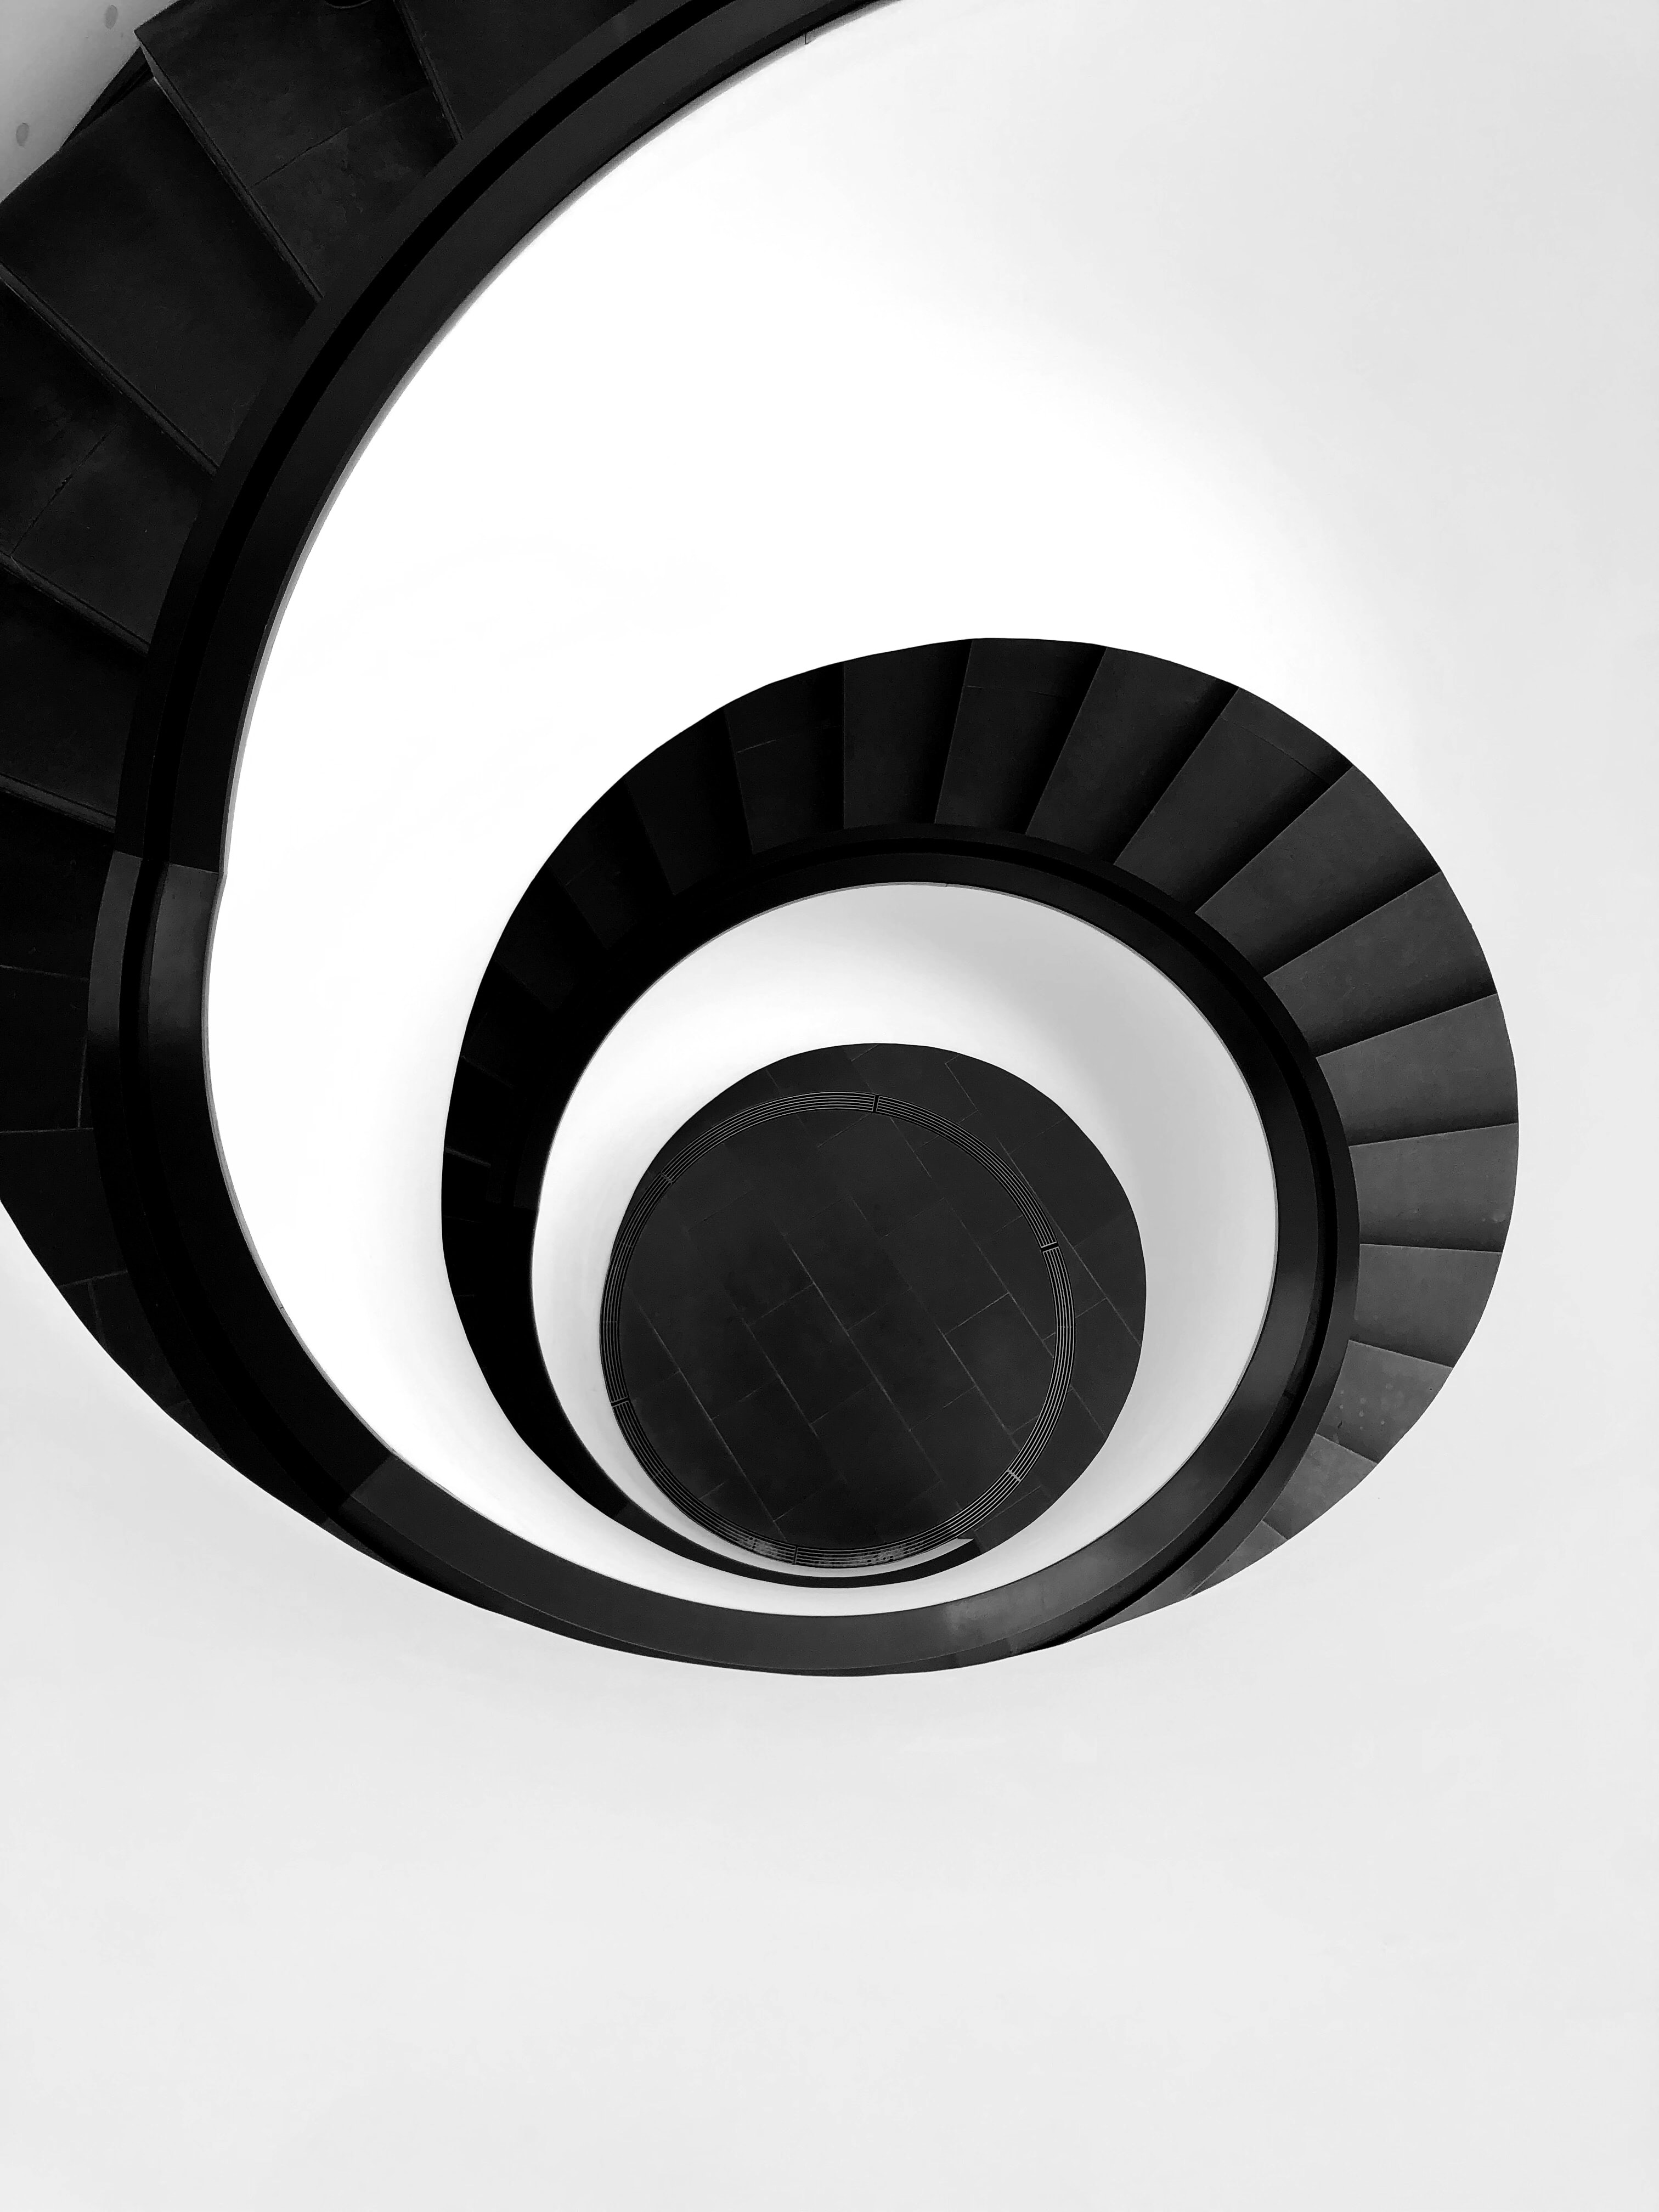
\includegraphics[width=0.4\textwidth,height=\textheight]{img/spiral-robin-schreiner-d8OiIdAdKNA-unsplash.jpg}

}

\caption{Og så videre}

\end{figure}

\hypertarget{data-frame}{%
\section{Data frame}\label{data-frame}}

Vi arbeider mest med datasett, og disse har en egen klasse i R, nemlig
\emph{data frame}. Jeg kommer ikke på noen god norsk oversettelse av
\emph{data frame}, så jeg bruker det engelske ordet. Dette fordi jeg på
engelsk ville skilt mellom \emph{datasets}, altså et datasett som kunne
finnes i ulike dataformater (\texttt{.sav}, \texttt{.csv},
\texttt{.xlsx}) og \emph{data frames}, altså en datastruktur i R.

\begin{Shaded}
\begin{Highlighting}[]
\CommentTok{\# En enkel data frame.}
\NormalTok{dat1 }\OtherTok{\textless{}{-}} \FunctionTok{data.frame}\NormalTok{(}
  \AttributeTok{personer =} \FunctionTok{c}\NormalTok{(}\StringTok{"Luke"}\NormalTok{, }\StringTok{"Han"}\NormalTok{, }\StringTok{"Darth"}\NormalTok{),}
  \AttributeTok{moral =} \FunctionTok{c}\NormalTok{(}\StringTok{"Bra"}\NormalTok{, }\StringTok{"Nja"}\NormalTok{, }\StringTok{"Dårlig"}\NormalTok{)}
\NormalTok{)}
\NormalTok{dat1}
\end{Highlighting}
\end{Shaded}

\begin{verbatim}
  personer  moral
1     Luke    Bra
2      Han    Nja
3    Darth Dårlig
\end{verbatim}

\begin{Shaded}
\begin{Highlighting}[]
\CommentTok{\# Vi kan lage et data frame via vektorer som er predefinerte,}
\CommentTok{\# så lenge begge har lik lengde.}
\NormalTok{dat2 }\OtherTok{\textless{}{-}} \FunctionTok{data.frame}\NormalTok{(}
  \AttributeTok{colA =}\NormalTok{ vektor1,}
  \AttributeTok{colB =}\NormalTok{ vektor2}
\NormalTok{)}
\NormalTok{dat2}
\end{Highlighting}
\end{Shaded}

\begin{verbatim}
  colA colB
1    1    A
2    2    B
3    3    C
\end{verbatim}

Det interessante med data frames er at de faktisk bare er
\textbf{lister}. Det vil si at mye av det vi veit om lister kan brukes
på data frames. Et data frame er strengt tatt bare ei liste med
vektorer. Hver vektor blir en \emph{kolonne} i data framen. Hva
representerer hver \textbf{rad}? Det er ikke gitt, men vi kan vanligvis
tenke på hver rad som en observasjon. Når vi prater om \emph{tidy data}
vil dette bli utdypa.

\begin{Shaded}
\begin{Highlighting}[]
\CommentTok{\# Sjekk ut første element av dat1}
\NormalTok{dat1[}\DecValTok{1}\NormalTok{]}
\end{Highlighting}
\end{Shaded}

\begin{verbatim}
  personer
1     Luke
2      Han
3    Darth
\end{verbatim}

Det er noen begrensninger eller krav ved datasett: hver kolonne må ha
lik lengde. Hvis ikke får du feilmelding.

\begin{Shaded}
\begin{Highlighting}[]
\NormalTok{dat3 }\OtherTok{\textless{}{-}} \FunctionTok{data.frame}\NormalTok{(}
  \AttributeTok{colA =} \FunctionTok{c}\NormalTok{(}\DecValTok{1}\NormalTok{, }\DecValTok{2}\NormalTok{, }\DecValTok{3}\NormalTok{, }\DecValTok{4}\NormalTok{),}
  \AttributeTok{colB =} \FunctionTok{c}\NormalTok{(}\DecValTok{5}\NormalTok{, }\DecValTok{6}\NormalTok{, }\DecValTok{7}\NormalTok{)}
\NormalTok{)}
\end{Highlighting}
\end{Shaded}

\begin{verbatim}
Error in data.frame(colA = c(1, 2, 3, 4), colB = c(5, 6, 7)): arguments imply differing number of rows: 4, 3
\end{verbatim}

R er snill og gir oss tydelig beskjed om hva som er galt i feilmeldinga.

En ting som er fint med alle disse R-pakkene, er at de ofte inkluderer
datasett som vi kan bruke for å illustrere pakkens funksjoner. Disse
datasetta ligger tilgjengelig på samme måte som funksjonene: man bare
skriver navnet dens for å påkalle den. La oss hente et datasett som
kommer fra \texttt{dplyr} (som er en del av \texttt{tidyverse}).

\begin{Shaded}
\begin{Highlighting}[]
\NormalTok{starwars}
\end{Highlighting}
\end{Shaded}

\begin{verbatim}
# A tibble: 87 x 14
   name        height  mass hair_~1 skin_~2 eye_c~3 birth~4 sex   gender homew~5
   <chr>        <int> <dbl> <chr>   <chr>   <chr>     <dbl> <chr> <chr>  <chr>  
 1 Luke Skywa~    172    77 blond   fair    blue       19   male  mascu~ Tatooi~
 2 C-3PO          167    75 <NA>    gold    yellow    112   none  mascu~ Tatooi~
 3 R2-D2           96    32 <NA>    white,~ red        33   none  mascu~ Naboo  
 4 Darth Vader    202   136 none    white   yellow     41.9 male  mascu~ Tatooi~
 5 Leia Organa    150    49 brown   light   brown      19   fema~ femin~ Aldera~
 6 Owen Lars      178   120 brown,~ light   blue       52   male  mascu~ Tatooi~
 7 Beru White~    165    75 brown   light   blue       47   fema~ femin~ Tatooi~
 8 R5-D4           97    32 <NA>    white,~ red        NA   none  mascu~ Tatooi~
 9 Biggs Dark~    183    84 black   light   brown      24   male  mascu~ Tatooi~
10 Obi-Wan Ke~    182    77 auburn~ fair    blue-g~    57   male  mascu~ Stewjon
# ... with 77 more rows, 4 more variables: species <chr>, films <list>,
#   vehicles <list>, starships <list>, and abbreviated variable names
#   1: hair_color, 2: skin_color, 3: eye_color, 4: birth_year, 5: homeworld
\end{verbatim}

Det kan føles rart å jobbe med data som vi ikke veit hvor ligger. Så jeg
kan plassere det explisitt i \textbf{miljøet} vårt (\emph{environment}),
ved å \emph{assigne} det.

\begin{Shaded}
\begin{Highlighting}[]
\CommentTok{\# Hvis du kjører denne koden vil du se at et objekt ved navn \textasciigrave{}starwars\textasciigrave{} dukker }
\CommentTok{\# opp i det globale miljøet i vinduet til høyre.}
\NormalTok{starwars }\OtherTok{\textless{}{-}}\NormalTok{ starwars}
\end{Highlighting}
\end{Shaded}

La oss bruke dette datasettet for å vise noen flere egenskaper ved R.
Men vent, er dette et \emph{data frame}?

\begin{Shaded}
\begin{Highlighting}[]
\NormalTok{starwars }\SpecialCharTok{\%\textgreater{}\%} \FunctionTok{class}\NormalTok{()}
\end{Highlighting}
\end{Shaded}

\begin{verbatim}
[1] "tbl_df"     "tbl"        "data.frame"
\end{verbatim}

\hypertarget{tibble}{%
\subsubsection{Tibble}\label{tibble}}

Som vi ser av sjekken over, har starwars tre klasser, hvor én av dem er
en \texttt{data.frame}. Til sammenlikning har de data framene vi lagde
tidligere bare én klasse:

\begin{Shaded}
\begin{Highlighting}[]
\NormalTok{dat1 }\SpecialCharTok{\%\textgreater{}\%} \FunctionTok{class}\NormalTok{()}
\end{Highlighting}
\end{Shaded}

\begin{verbatim}
[1] "data.frame"
\end{verbatim}

Så hva er en \texttt{tibble}? Kort fortalt er en tibble en forbedra
versjon av et data frame. Tibbles kommer fra pakka \texttt{tibble} som,
du gjetta riktig, er en del av \texttt{tidyverse}. En fordel med tibbles
er at de \emph{printer bedre til konsollen}. Spesielt store datasett
(vår spesialitet) blir mer leselig i tibbles. Når vi arbeider med
\texttt{tidyverse} vil mange av data framene våre bli til tibbles via
funksjonene deres. Vi trenger altså sjelden tenke mye på dette. Tibbles
arver også klassen \texttt{data.frame} som vi så over, så de fleste
funksjoner som ikke har hørt om tibbles vil også funke på dem. Flere
fordeler forklares i
\href{https://tibble.tidyverse.org/}{dokumentasjonen til pakka}.

For å oppsummere: du trenger sjelden bry deg om du jobber med tibbles
eller data frames. Jeg nevner det her fordi du kanskje vil lure på
hvorfor vi noen får \texttt{tibble}-objekter.

\hypertarget{tilbake-til-elementer}{%
\subsection{Tilbake til elementer}\label{tilbake-til-elementer}}

Nå som vi har tilgang til et større datasett kan vi utforske litt mer
hvordan vi arbeider med, nettopp, større datasett. Datasettet
\texttt{starwars} inneholder informasjon om dokumentarserien \emph{Star
Wars}, som omhandla livet i gamle dager, i en galakse langt, langt vekk.

\begin{Shaded}
\begin{Highlighting}[]
\NormalTok{starwars}
\end{Highlighting}
\end{Shaded}

\begin{verbatim}
# A tibble: 87 x 14
   name        height  mass hair_~1 skin_~2 eye_c~3 birth~4 sex   gender homew~5
   <chr>        <int> <dbl> <chr>   <chr>   <chr>     <dbl> <chr> <chr>  <chr>  
 1 Luke Skywa~    172    77 blond   fair    blue       19   male  mascu~ Tatooi~
 2 C-3PO          167    75 <NA>    gold    yellow    112   none  mascu~ Tatooi~
 3 R2-D2           96    32 <NA>    white,~ red        33   none  mascu~ Naboo  
 4 Darth Vader    202   136 none    white   yellow     41.9 male  mascu~ Tatooi~
 5 Leia Organa    150    49 brown   light   brown      19   fema~ femin~ Aldera~
 6 Owen Lars      178   120 brown,~ light   blue       52   male  mascu~ Tatooi~
 7 Beru White~    165    75 brown   light   blue       47   fema~ femin~ Tatooi~
 8 R5-D4           97    32 <NA>    white,~ red        NA   none  mascu~ Tatooi~
 9 Biggs Dark~    183    84 black   light   brown      24   male  mascu~ Tatooi~
10 Obi-Wan Ke~    182    77 auburn~ fair    blue-g~    57   male  mascu~ Stewjon
# ... with 77 more rows, 4 more variables: species <chr>, films <list>,
#   vehicles <list>, starships <list>, and abbreviated variable names
#   1: hair_color, 2: skin_color, 3: eye_color, 4: birth_year, 5: homeworld
\end{verbatim}

På tide å utforske. Vi kan henvise til spesifikke celler via x- og
y-koordinater.

\begin{Shaded}
\begin{Highlighting}[]
\CommentTok{\# Vi kan finne en nøyaktig celle ved å henvise til x{-} og y{-}koordinatene}
\NormalTok{starwars[}\DecValTok{2}\NormalTok{, }\DecValTok{1}\NormalTok{]}
\end{Highlighting}
\end{Shaded}

\begin{verbatim}
# A tibble: 1 x 1
  name 
  <chr>
1 C-3PO
\end{verbatim}

\begin{Shaded}
\begin{Highlighting}[]
\NormalTok{starwars[}\DecValTok{5}\NormalTok{, }\DecValTok{4}\NormalTok{]}
\end{Highlighting}
\end{Shaded}

\begin{verbatim}
# A tibble: 1 x 1
  hair_color
  <chr>     
1 brown     
\end{verbatim}

\begin{Shaded}
\begin{Highlighting}[]
\CommentTok{\# Vi kan få tak i en serie med elementer via \textasciigrave{}:\textasciigrave{}}
\NormalTok{starwars[}\DecValTok{1}\SpecialCharTok{:}\DecValTok{3}\NormalTok{]}
\end{Highlighting}
\end{Shaded}

\begin{verbatim}
# A tibble: 87 x 3
   name               height  mass
   <chr>               <int> <dbl>
 1 Luke Skywalker        172    77
 2 C-3PO                 167    75
 3 R2-D2                  96    32
 4 Darth Vader           202   136
 5 Leia Organa           150    49
 6 Owen Lars             178   120
 7 Beru Whitesun lars    165    75
 8 R5-D4                  97    32
 9 Biggs Darklighter     183    84
10 Obi-Wan Kenobi        182    77
# ... with 77 more rows
\end{verbatim}

\begin{Shaded}
\begin{Highlighting}[]
\CommentTok{\# Vi kan gjøre et utvalg av celler ved å definere både x og y som en serie}
\NormalTok{starwars[}\DecValTok{2}\SpecialCharTok{:}\DecValTok{5}\NormalTok{, }\DecValTok{6}\SpecialCharTok{:}\DecValTok{9}\NormalTok{]}
\end{Highlighting}
\end{Shaded}

\begin{verbatim}
# A tibble: 4 x 4
  eye_color birth_year sex    gender   
  <chr>          <dbl> <chr>  <chr>    
1 yellow         112   none   masculine
2 red             33   none   masculine
3 yellow          41.9 male   masculine
4 brown           19   female feminine 
\end{verbatim}

Det er upraktisk å skulle huske indekser til alt. Heldigvis kan vi
henvise til kolonner dersom de er navngitt, slik som her:

\begin{Shaded}
\begin{Highlighting}[]
\NormalTok{starwars[}\StringTok{"eye\_color"}\NormalTok{]}
\end{Highlighting}
\end{Shaded}

\begin{verbatim}
# A tibble: 87 x 1
   eye_color
   <chr>    
 1 blue     
 2 yellow   
 3 red      
 4 yellow   
 5 brown    
 6 blue     
 7 blue     
 8 red      
 9 brown    
10 blue-gray
# ... with 77 more rows
\end{verbatim}

\begin{Shaded}
\begin{Highlighting}[]
\CommentTok{\# En nyttig funksjon for å finne navna til alle kolonnene (variablene) er:}
\FunctionTok{colnames}\NormalTok{(starwars)}
\end{Highlighting}
\end{Shaded}

\begin{verbatim}
 [1] "name"       "height"     "mass"       "hair_color" "skin_color"
 [6] "eye_color"  "birth_year" "sex"        "gender"     "homeworld" 
[11] "species"    "films"      "vehicles"   "starships" 
\end{verbatim}

\begin{Shaded}
\begin{Highlighting}[]
\NormalTok{starwars[}\StringTok{"species"}\NormalTok{]}
\end{Highlighting}
\end{Shaded}

\begin{verbatim}
# A tibble: 87 x 1
   species
   <chr>  
 1 Human  
 2 Droid  
 3 Droid  
 4 Human  
 5 Human  
 6 Human  
 7 Human  
 8 Droid  
 9 Human  
10 Human  
# ... with 77 more rows
\end{verbatim}

Et alterntiv til klammeparantesen er å bruke operatoren `\$´.

\begin{Shaded}
\begin{Highlighting}[]
\CommentTok{\# Her trenger man ikke hermetegn, med mindre kolonna har mellomrom.}
\NormalTok{starwars}\SpecialCharTok{$}\NormalTok{name}
\end{Highlighting}
\end{Shaded}

\begin{verbatim}
 [1] "Luke Skywalker"        "C-3PO"                 "R2-D2"                
 [4] "Darth Vader"           "Leia Organa"           "Owen Lars"            
 [7] "Beru Whitesun lars"    "R5-D4"                 "Biggs Darklighter"    
[10] "Obi-Wan Kenobi"        "Anakin Skywalker"      "Wilhuff Tarkin"       
[13] "Chewbacca"             "Han Solo"              "Greedo"               
[16] "Jabba Desilijic Tiure" "Wedge Antilles"        "Jek Tono Porkins"     
[19] "Yoda"                  "Palpatine"             "Boba Fett"            
[22] "IG-88"                 "Bossk"                 "Lando Calrissian"     
[25] "Lobot"                 "Ackbar"                "Mon Mothma"           
[28] "Arvel Crynyd"          "Wicket Systri Warrick" "Nien Nunb"            
[31] "Qui-Gon Jinn"          "Nute Gunray"           "Finis Valorum"        
[34] "Jar Jar Binks"         "Roos Tarpals"          "Rugor Nass"           
[37] "Ric Olié"              "Watto"                 "Sebulba"              
[40] "Quarsh Panaka"         "Shmi Skywalker"        "Darth Maul"           
[43] "Bib Fortuna"           "Ayla Secura"           "Dud Bolt"             
[46] "Gasgano"               "Ben Quadinaros"        "Mace Windu"           
[49] "Ki-Adi-Mundi"          "Kit Fisto"             "Eeth Koth"            
[52] "Adi Gallia"            "Saesee Tiin"           "Yarael Poof"          
[55] "Plo Koon"              "Mas Amedda"            "Gregar Typho"         
[58] "Cordé"                 "Cliegg Lars"           "Poggle the Lesser"    
[61] "Luminara Unduli"       "Barriss Offee"         "Dormé"                
[64] "Dooku"                 "Bail Prestor Organa"   "Jango Fett"           
[67] "Zam Wesell"            "Dexter Jettster"       "Lama Su"              
[70] "Taun We"               "Jocasta Nu"            "Ratts Tyerell"        
[73] "R4-P17"                "Wat Tambor"            "San Hill"             
[76] "Shaak Ti"              "Grievous"              "Tarfful"              
[79] "Raymus Antilles"       "Sly Moore"             "Tion Medon"           
[82] "Finn"                  "Rey"                   "Poe Dameron"          
[85] "BB8"                   "Captain Phasma"        "Padmé Amidala"        
\end{verbatim}

\begin{Shaded}
\begin{Highlighting}[]
\NormalTok{starwars}\SpecialCharTok{$}\StringTok{"name"}
\end{Highlighting}
\end{Shaded}

\begin{verbatim}
 [1] "Luke Skywalker"        "C-3PO"                 "R2-D2"                
 [4] "Darth Vader"           "Leia Organa"           "Owen Lars"            
 [7] "Beru Whitesun lars"    "R5-D4"                 "Biggs Darklighter"    
[10] "Obi-Wan Kenobi"        "Anakin Skywalker"      "Wilhuff Tarkin"       
[13] "Chewbacca"             "Han Solo"              "Greedo"               
[16] "Jabba Desilijic Tiure" "Wedge Antilles"        "Jek Tono Porkins"     
[19] "Yoda"                  "Palpatine"             "Boba Fett"            
[22] "IG-88"                 "Bossk"                 "Lando Calrissian"     
[25] "Lobot"                 "Ackbar"                "Mon Mothma"           
[28] "Arvel Crynyd"          "Wicket Systri Warrick" "Nien Nunb"            
[31] "Qui-Gon Jinn"          "Nute Gunray"           "Finis Valorum"        
[34] "Jar Jar Binks"         "Roos Tarpals"          "Rugor Nass"           
[37] "Ric Olié"              "Watto"                 "Sebulba"              
[40] "Quarsh Panaka"         "Shmi Skywalker"        "Darth Maul"           
[43] "Bib Fortuna"           "Ayla Secura"           "Dud Bolt"             
[46] "Gasgano"               "Ben Quadinaros"        "Mace Windu"           
[49] "Ki-Adi-Mundi"          "Kit Fisto"             "Eeth Koth"            
[52] "Adi Gallia"            "Saesee Tiin"           "Yarael Poof"          
[55] "Plo Koon"              "Mas Amedda"            "Gregar Typho"         
[58] "Cordé"                 "Cliegg Lars"           "Poggle the Lesser"    
[61] "Luminara Unduli"       "Barriss Offee"         "Dormé"                
[64] "Dooku"                 "Bail Prestor Organa"   "Jango Fett"           
[67] "Zam Wesell"            "Dexter Jettster"       "Lama Su"              
[70] "Taun We"               "Jocasta Nu"            "Ratts Tyerell"        
[73] "R4-P17"                "Wat Tambor"            "San Hill"             
[76] "Shaak Ti"              "Grievous"              "Tarfful"              
[79] "Raymus Antilles"       "Sly Moore"             "Tion Medon"           
[82] "Finn"                  "Rey"                   "Poe Dameron"          
[85] "BB8"                   "Captain Phasma"        "Padmé Amidala"        
\end{verbatim}

Som du begynner å skjønne er det flere veier til Rom. Klammeparantesen
og \texttt{\$} har tildels overlappende funksjoner. De har likevel sine
unike bruksområder. De vil vi lære å anerkjenne etter hvert som vi
arbeider med dem. En nyttig ting med \texttt{{[}{]}} er at vi kan bruke
det som et enkelt filter.

\begin{Shaded}
\begin{Highlighting}[]
\CommentTok{\# Velg kun de karakterene som er menneske}
\NormalTok{starwars[starwars}\SpecialCharTok{$}\NormalTok{species }\SpecialCharTok{==} \StringTok{"Human"}\NormalTok{, ]}
\end{Highlighting}
\end{Shaded}

\begin{verbatim}
# A tibble: 39 x 14
   name        height  mass hair_~1 skin_~2 eye_c~3 birth~4 sex   gender homew~5
   <chr>        <int> <dbl> <chr>   <chr>   <chr>     <dbl> <chr> <chr>  <chr>  
 1 Luke Skywa~    172    77 blond   fair    blue       19   male  mascu~ Tatooi~
 2 Darth Vader    202   136 none    white   yellow     41.9 male  mascu~ Tatooi~
 3 Leia Organa    150    49 brown   light   brown      19   fema~ femin~ Aldera~
 4 Owen Lars      178   120 brown,~ light   blue       52   male  mascu~ Tatooi~
 5 Beru White~    165    75 brown   light   blue       47   fema~ femin~ Tatooi~
 6 Biggs Dark~    183    84 black   light   brown      24   male  mascu~ Tatooi~
 7 Obi-Wan Ke~    182    77 auburn~ fair    blue-g~    57   male  mascu~ Stewjon
 8 Anakin Sky~    188    84 blond   fair    blue       41.9 male  mascu~ Tatooi~
 9 Wilhuff Ta~    180    NA auburn~ fair    blue       64   male  mascu~ Eriadu 
10 Han Solo       180    80 brown   fair    brown      29   male  mascu~ Corell~
# ... with 29 more rows, 4 more variables: species <chr>, films <list>,
#   vehicles <list>, starships <list>, and abbreviated variable names
#   1: hair_color, 2: skin_color, 3: eye_color, 4: birth_year, 5: homeworld
\end{verbatim}

Dette er noe knotete: Du må gjengi datasettnavnet inni klamma, og du må
huske på kommaet for å implisitt velge alle rader. Dessuten vil du bare
få treff på nøyaktig det samme. Hvis noen har en \texttt{species} som er
skrevet f.eks. \texttt{human} eller \texttt{human/alien} vil vi ikke få
treff. Hvis det bare hadde fantes en smartere implementering av dette
filteret \ldots{}

Og det gjør det! I, nettopp, \texttt{tidyverse}!

\includegraphics[width=0.3\textwidth,height=\textheight]{img/tidyverse-logo.png}

På tampen, noen nyttige digresjoner.

\hypertarget{digresjoner}{%
\subsection{Digresjoner}\label{digresjoner}}

\hypertarget{sec-navngitt-vektor}{%
\subsubsection{Navngitte lister/vektorer}\label{sec-navngitt-vektor}}

Vi returnerer til lister og vektorer. Tenk på de vi lagde tidligere:

\begin{Shaded}
\begin{Highlighting}[]
\NormalTok{vektor1}
\end{Highlighting}
\end{Shaded}

\begin{verbatim}
[1] 1 2 3
\end{verbatim}

\begin{Shaded}
\begin{Highlighting}[]
\NormalTok{liste1}
\end{Highlighting}
\end{Shaded}

\begin{verbatim}
[[1]]
[1] 1

[[2]]
[1] "B"

[[3]]
[1] 3

[[4]]
[1] "D"

[[5]]
[1] 5
\end{verbatim}

De er enkle. Kan vi gjøre dem \ldots{} mer komplisert? Så klart. Noe som
ofte vil være nyttig for oss er det å bruke \textbf{navngitte vektorer
eller lister} (\emph{named vector/named list}). Hva er det? Det er en
vektor eller liste hvor \emph{hvert element har et navn}. La oss se noen
eksempler. (Jeg viser bare for vektorer, men det samme gjelder for
lister.)

\begin{Shaded}
\begin{Highlighting}[]
\NormalTok{navngitt\_vektor }\OtherTok{\textless{}{-}} \FunctionTok{c}\NormalTok{(}\StringTok{"navn"} \OtherTok{=} \StringTok{"Arnold"}\NormalTok{,}
                     \StringTok{"hilsen"} \OtherTok{=} \StringTok{"hey"}\NormalTok{,}
                     \StringTok{"venn"} \OtherTok{=} \StringTok{"Gerald"}\NormalTok{)}

\CommentTok{\# Nå har hvert element i vektoren et navn}
\NormalTok{navngitt\_vektor}
\end{Highlighting}
\end{Shaded}

\begin{verbatim}
    navn   hilsen     venn 
"Arnold"    "hey" "Gerald" 
\end{verbatim}

\begin{Shaded}
\begin{Highlighting}[]
\CommentTok{\# Sammenlikn med den tidligere, navnløse vektoren. }
\NormalTok{vektor2}
\end{Highlighting}
\end{Shaded}

\begin{verbatim}
[1] "A" "B" "C"
\end{verbatim}

\begin{Shaded}
\begin{Highlighting}[]
\CommentTok{\# Vi kan også bruke funksjonen \textasciigrave{}setNames()\textasciigrave{} til å gi navn. Nyttig hvis vi har}
\CommentTok{\# navna lagra i en annen vektor/liste}
\NormalTok{navn }\OtherTok{\textless{}{-}} \FunctionTok{c}\NormalTok{(}\StringTok{"Første"}\NormalTok{, }\StringTok{"Andre"}\NormalTok{, }\StringTok{"Tredje"}\NormalTok{)}

\FunctionTok{setNames}\NormalTok{(vektor2, navn)}
\end{Highlighting}
\end{Shaded}

\begin{verbatim}
Første  Andre Tredje 
   "A"    "B"    "C" 
\end{verbatim}

\begin{Shaded}
\begin{Highlighting}[]
\CommentTok{\# Men {-}{-}{-} hvor har navna våre blitt av??}
\NormalTok{vektor2}
\end{Highlighting}
\end{Shaded}

\begin{verbatim}
[1] "A" "B" "C"
\end{verbatim}

\begin{Shaded}
\begin{Highlighting}[]
\CommentTok{\# Vi må huske å bruke *assignment* for å large det vi gjør}
\NormalTok{vektor2 }\OtherTok{\textless{}{-}} \FunctionTok{setNames}\NormalTok{(vektor2, navn)}
\NormalTok{vektor2}
\end{Highlighting}
\end{Shaded}

\begin{verbatim}
Første  Andre Tredje 
   "A"    "B"    "C" 
\end{verbatim}

Hvorfor er det nyttig? Navngitte vektorer og lister er nyttig fordi det
er mange funskjoner i spesielt \texttt{tidyverse} som nyttiggjør seg av
dem. Når man for eksempel bruker \texttt{rename()} til å endre navn på
variabler kan man sende en navngitt vektor for å endre mange navn på en
gang. Dette gjør at vi mer programmatisk kan endre navn istedenfor å
skrive hvert ledd. Når vi har mange ledd, slik som i navn på plansoner
og kommunenummer, blir dette svært nyttig.

Forresten, her er en ting jeg ofte brenner meg på: Når du bruker
\texttt{setNames()} kommer elementnavna \emph{etter} elementene. Når du
navngir elementene mens du lager vektoren/lista, kommer elemtnnavna
\emph{først}. Du ser det i eksemplene over.

\hypertarget{assignment-og--}{%
\subsubsection{\texorpdfstring{Assignment (\texttt{=} og
\texttt{\textless{}-})}{Assignment (= og \textless-)}}\label{assignment-og--}}

Kanskje dere føler dere lurt av noe jeg så tidligere.

\begin{quote}
Derfor bruker jeg alltid \texttt{\textless{}-}, og anbefaler deg det
også.
\end{quote}

Og litt lengre ned viser

\begin{Shaded}
\begin{Highlighting}[]
\CommentTok{\# En enkel data frame.}
\NormalTok{dat1 }\OtherTok{\textless{}{-}} \FunctionTok{data.frame}\NormalTok{(}
  \AttributeTok{personer =} \FunctionTok{c}\NormalTok{(}\StringTok{"Luke"}\NormalTok{, }\StringTok{"Han"}\NormalTok{, }\StringTok{"Darth"}\NormalTok{),}
  \AttributeTok{moral =} \FunctionTok{c}\NormalTok{(}\StringTok{"Bra"}\NormalTok{, }\StringTok{"Nja"}\NormalTok{, }\StringTok{"Dårlig"}\NormalTok{)}
\NormalTok{)}
\NormalTok{dat1}
\end{Highlighting}
\end{Shaded}

\begin{verbatim}
  personer  moral
1     Luke    Bra
2      Han    Nja
3    Darth Dårlig
\end{verbatim}

Men her bruker jeg jo \texttt{=} som assignment. Hva skjer?

Poenget her er at jeg bruker \texttt{=} inni funksjonens argumenter.
\texttt{data.frame()} er en funksjon, og jeg definerer her hva som skal
være kolonnene i datasettet mitt. Så bruker jeg \texttt{\textless{}-}
til å \emph{assigne} det som funksjonen \texttt{data.frame()}
returnerer. Forvirra? På generelt grunnlag kan vi si at vi bruker
\texttt{=} inni funksjoner, og \texttt{\textless{}-} utafor\footnote{Når
  vi seinere definerer våre egne funksjoner vil du se at det jeg sier
  her ikke er helt korrekt, men det er en grei heuristikk fram til da.}.

Forresten, hvorfor prøver vi ikke bare å bruke \texttt{\textless{}-}
inni funksjonen og ser hva som skjer?

\begin{Shaded}
\begin{Highlighting}[]
\CommentTok{\# Funker ikke}
\NormalTok{dat1x }\OtherTok{\textless{}{-}} \FunctionTok{data.frame}\NormalTok{(}
\NormalTok{  personer }\OtherTok{\textless{}{-}} \FunctionTok{c}\NormalTok{(}\StringTok{"Luke"}\NormalTok{, }\StringTok{"Han"}\NormalTok{, }\StringTok{"Darth"}\NormalTok{),}
\NormalTok{  moral }\OtherTok{\textless{}{-}} \FunctionTok{c}\NormalTok{(}\StringTok{"Bra"}\NormalTok{, }\StringTok{"Nja"}\NormalTok{, }\StringTok{"Dårlig"}\NormalTok{)}
\NormalTok{)}

\NormalTok{dat1}
\end{Highlighting}
\end{Shaded}

\begin{verbatim}
  personer  moral
1     Luke    Bra
2      Han    Nja
3    Darth Dårlig
\end{verbatim}

\begin{Shaded}
\begin{Highlighting}[]
\NormalTok{dat1x}
\end{Highlighting}
\end{Shaded}

\begin{verbatim}
  personer....c..Luke....Han....Darth.. moral....c..Bra....Nja....Dårlig..
1                                  Luke                                Bra
2                                   Han                                Nja
3                                 Darth                             Dårlig
\end{verbatim}

Hvis vi sammenlikner de to datasetta ser vi at det funker \ldots{} på en
måte. Oppsettet blir likt, men vi mister navnet på kolonnene.



\end{document}
